
\documentclass[12pt, a4paper]{article}


%%%%%%%%%% Import Packages %%%%%%%%%

\usepackage[margin=2cm]{geometry} % 2cm margins
\usepackage{amsmath,amsthm,amssymb} % AMS math environment
\usepackage{fontspec}   % font setting
\usepackage{type1cm}    % fontsize setting
\usepackage{titlesec}   % section, subsection ... font setting
\usepackage{titling}    % title setting
\usepackage{fancyhdr}   % header and footer
\usepackage{enumerate}  % improving enumerate
\usepackage{stmaryrd}   % some math fonts
\usepackage[square, comma, numbers, sort&compress]{natbib} % bibliography
\usepackage[usenames, dvipsnames]{color} % to use colors
\usepackage{hyperref}   % advanced reference

%%%%%%%%%%% For figures %%%%%%%%%%
\usepackage{graphicx}    % insert figures
\usepackage{float}       % fix the position of the figure with [H]

%%%%%%%%%% Table and caption packages %%%%%%%%%%%
\usepackage{booktabs} % toprule, bottomrule ...
\usepackage{tabu}
\usepackage{multirow}
\usepackage{tabularx}
\usepackage{caption}
\usepackage{caption3}
\usepackage{subcaption}

%%%%%%%%%% Chinese Environment %%%%%%%%%%
\usepackage[AutoFakeBold, CheckSingle, CJKmath]{xeCJK}  % xelatex Chinese
\usepackage{CJKulem}	% Chinese character decoration


%%%%%%%%%% Page settings %%%%%%%%%% 
\setlength{\headheight}{15pt}  % with titling
\setlength{\droptitle}{-1.5cm} % white space before the title
\parindent=24pt % indent spacing
\parskip=0.8em  % spacing between two paragraphs


%%%%%%%%%% Math display spacing (gather, equation, ...) %%%%%%%%%%
\makeatletter
\g@addto@macro\normalsize{%
  \setlength{\abovedisplayskip}{-8pt}
  \setlength{\belowdisplayskip}{4pt}
  \setlength{\abovedisplayshortskip}{-8pt}
  \setlength{\belowdisplayshortskip}{4pt}
}


%%%%%%%%%% Figure caption %%%%%%%%%%
\captionsetup[figure]{
 	font = small,
	name = \textsc{Figure},
	justification = justified, % caption as normal paragraph
    labelsep = colon, % Figure: ...
	skip = \medskipamount} % space between caption and image
\captionsetup[sub]{font = small, belowskip = 2pt}
\setlength{\belowcaptionskip}{-8pt}

%%%%%%%%%% Figure position %%%%%%%%%%
\graphicspath{
{../figures/},
}


%%%%%%%%%% Table settings %%%%%%%%%%
\captionsetup[table]{
  parskip = 20pt,
  format = hang,
  font = small,
  name = \textsc{Table},
  justification = justified,
  skip = \medskipamount,
  singlelinecheck = false
}
\renewcommand{\arraystretch}{1.2}
\tabcolsep = 10pt


%%%%%%%%%% Reference settings %%%%%%%%%%
\hypersetup{
unicode=true, 
bookmarksdepth=-1, 
pdfborder={0 0 0}, 
colorlinks=true, 
linkcolor=RoyalBlue,
citecolor=blue
}


\begin{document}

%mainfile: Networks.tex

\pagestyle{fancy} 
\lhead{Atelier Nueromodélisation, 2017}
\rhead{Problem set \#4}
\rfoot{\thepage}
\cfoot{}
\lfoot{~\theauthor}
\renewcommand{\headrulewidth}{0.4pt}
\renewcommand{\footrulewidth}{0.4pt}


\title{Problem Set \#4: Networks \vspace{-0.5em}}
%\preauthor{} \postauthor{} 
\author{Hsieh Yu-Guan}
\date{\today}
\maketitle

\thispagestyle{fancy}

\section*{Introduction}

Besides studying the strucutre and function of a single neuron, it's also
important to understand what may happen when neurons communicate between them.
In this report we'll thus look at some simple models of neural networks.
What will be their dynamics and expressive power? 
(P.S. we'll ignore all physical units for the whole report.)

\section{Some simple networks}

\subsection{Neuron with autapse}

Let's start by working on the simplest model that one can ever imagine:
there's only one neuron in the network, and its output feeds back onto 
itself via a synapse (such a synapse is called an ``autapse''). 
We note $x$ the neuron's firing rate, and it obeys the equation

\[\dot{x}(t) = -x(t) + f(wx(t)+I)\]

\noindent
where $w = 0.04$ is the strength of the synaptic connection and $I = -2$ 
is the external (and inhibitory) background input which is constant.
Finally, $f$ is the input-output (or activation) function of the neuron having
a sigmoidal form and is given by

\[f(s) = 50(1 + \tanh(s))\]

\noindent
where $s$ is the total input of the neuron.

To see that $f$ is indeed a sigmoidal function, we plot it for the range 
$s \in [-10, 10]$ as shown in \autoref{fig: activate}. Next, we plot the
derivative of the firing rate $\dot{x}$ as a function of $x$ 
(\autoref{fig: x_derivative}). The form should be easily predictable.
The function $f$ is first stretched out and then shifted to the right,
before we finally add the linear function $x \mapsto -x$ to it.

We observe three zero-crossings in this graph. Let's call them respectively
$x_1$, $x_2$ and $x_3$ with $x_1 < x_2 < x_3$. In fact we get $x_1 \sim 2$,
$x_2 = 50$ and $x_3 \sim 98$. They are the fixed points of the dynamics.
However, $x_1$ and $x_3$ are stable while $x_2$ is unstable.
We can see that if $x$ lies between $x_1$ and $x_2$, $\dot{x}$ is negative
so $x$ will be ``attract'' to $x_1$, and if $x$ is smaller than $x_1$,
$\dot{x}$ is positive and $x$ will converge to $x_1$. The same analysis
works for $x_3$.

\newpage

\vspace{-1em}
\begin{figure}[H]
  \centering
  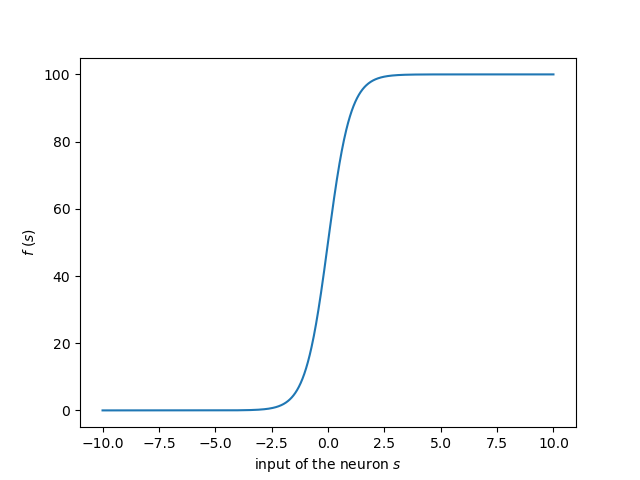
\includegraphics[width=0.7\linewidth]{autapse1}
  \caption{The activtion function $f$ of the neuron}
  \label{fig: activate}
\end{figure}

\vspace{-1em}
\begin{figure}[H]
  \centering
  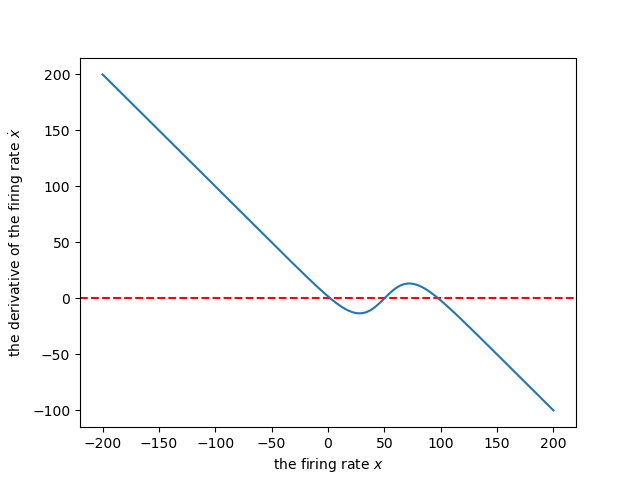
\includegraphics[width=0.7\linewidth]{autapse2}
  \caption{$\dot(x)$ as a function of $x$}
  \label{fig: x_derivative}
\end{figure}

Now we'll simulate the dynamics of the system by taking a time step 
$\Delta t = 0.1$ and a total time period $T = 100$. First consider
$x(0) = 49$.

\vspace{-1em}
\begin{figure}[H]
  \centering
  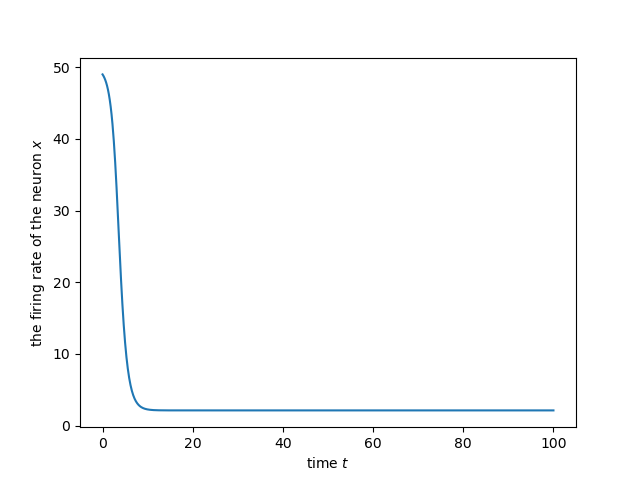
\includegraphics[width=0.7\linewidth]{autapse3}
  \caption{The evolution of $x$ for $x(0) = 49$}
\end{figure}

\noindent
As predicted before $x$ is attracted to the dynamics attractor $x_1$.
We redo the simulation for $x(0) = 50$.

\vspace{-1em}
\begin{figure}[H]
  \centering
  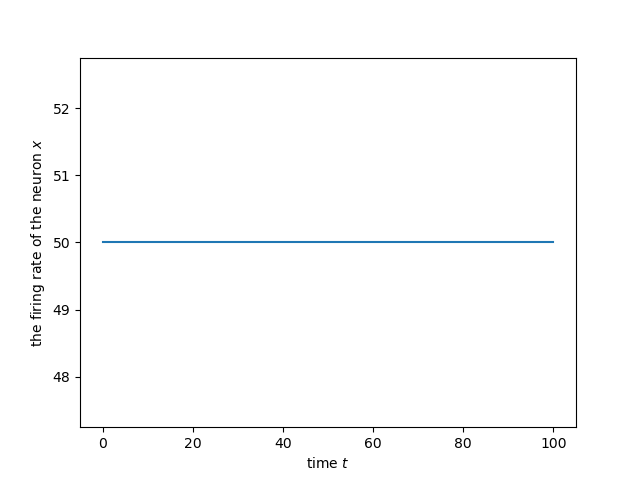
\includegraphics[width=0.7\linewidth]{autapse4}
  \caption{The evolution of $x$ for $x(0) = 50$}
\end{figure}

\noindent
This time since 50 is itself a fixed point of the dynamics, the system 
is at equilibrium and the solution doesn't change with time (though 50
is a repeller). Finally let $x(0) = 51$.

\vspace{-1em}
\begin{figure}[H]
  \centering
  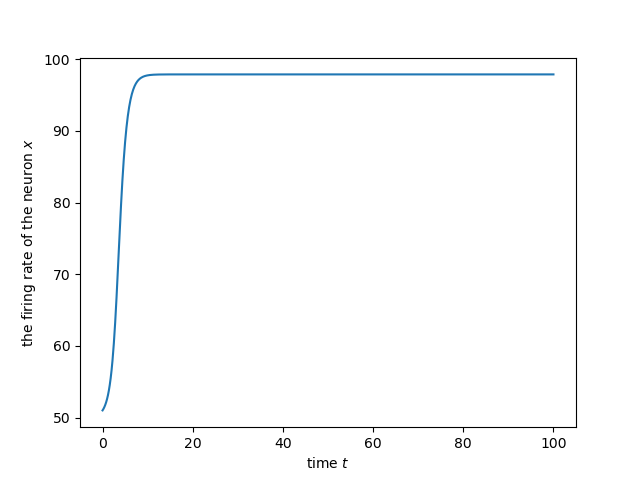
\includegraphics[width=0.7\linewidth]{autapse5}
  \caption{The evolution of $x$ for $x(0) = 51$}
\end{figure}

\noindent
It's the symmetry of the case $x(0) = 49$. Between the repeller $x_2$ and
the attractor $x_3$, $x$ evolves towards $x_3$.

We then add noise to the system, so the differential equation becomes

\[\dot{x}(t) = -x(t) + f(wx(t)+I) + \sigma\eta(t)\]

\noindent
where $\sigma(t)$ is Gaussian white noise with varaiance 1. First we suppose 
$\sigma = 5$ and we simulate for $x(0) = 49$.

\vspace{-1em}
\begin{figure}[H]
  \centering
  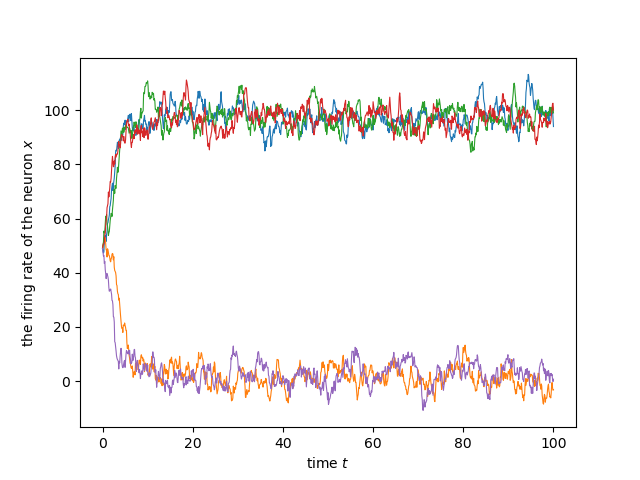
\includegraphics[width=0.7\linewidth]{autapse6}
  \caption{The evolution of $x$ with noise $\sigma = 5$ for $x(0) = 49$}
\end{figure}

We see that there are two different scinarios. With noise we can no longer
ensure that the system will converge towards $x_1$. Since the evolutions of
the system are very different for $x < 50$ and $x > 50$, and 49 is close
to 50, slight noise in the model may lead to totaly distinct results. This can
be again shown for $x(0) = 50$ and $x(0) = 51$.

\vspace{-1em}
\begin{figure}[H]
  \centering
  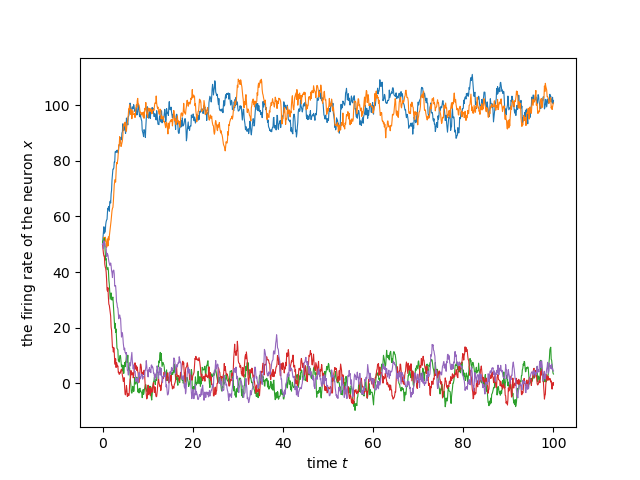
\includegraphics[width=0.7\linewidth]{autapse7}
  \caption{The evolution of $x$ with noise $\sigma = 5$ for $x(0) = 50$}
\end{figure}

\vspace{-1em}
\begin{figure}[H]
  \centering
  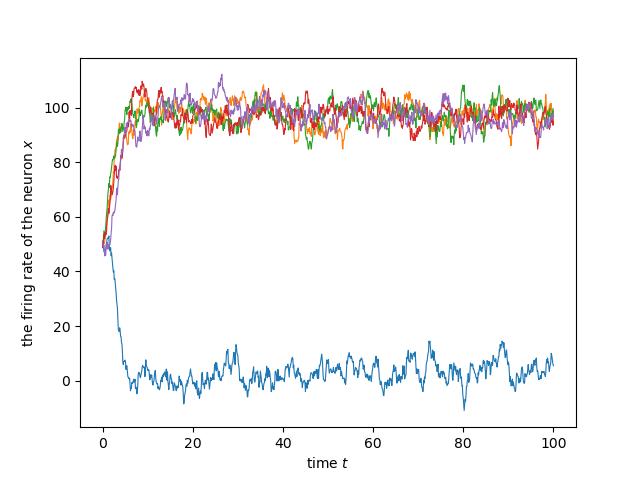
\includegraphics[width=0.7\linewidth]{autapse8}
  \caption{The evolution of $x$ with noise $\sigma = 5$ for $x(0) = 51$}
\end{figure}

Also notice that for $x(0) = 50$, $x$ will not stay anymore at the value 50 
because as mentioned before, $x_2 = 50$ is a repeller. In a model with noise,
the probability that $x$ is always 50 becomes null. 

In all the above examples, though noise can have great influence on the 
evolution of the system, once $x$ gets far enough from $x_2$, the evolution
is still mainly dominated by the drift term $-x(t) + f(wx(t)+I)$.
Nonetheless, this is not the case for a greater noise level, for example,
when $\sigma = 80$, as shown in the top of the next page.

\vspace{-1em}
\begin{figure}[H]
  \centering
  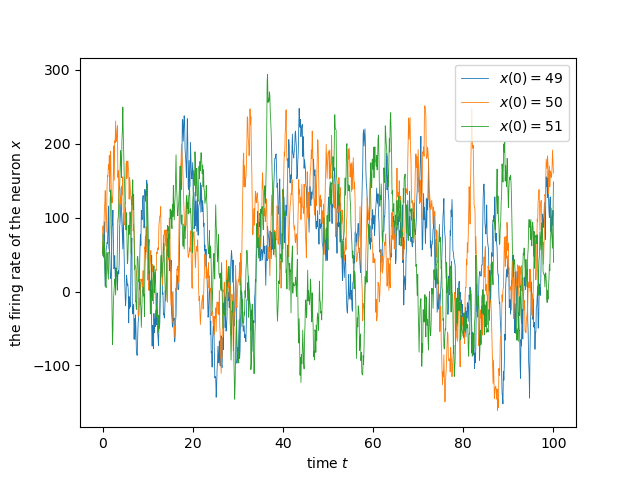
\includegraphics[width=0.7\linewidth]{autapse9}
  \caption
    {The evolution of $x$ with noise $\sigma = 80$ for $x(0) = 49, 50, 51$}
\end{figure}

As the resulting curves follow almost the same pattern for different 
initial values of $x$, I plot all of them on the same graph. It's not worth
it to plot several simulations for a same $x(0)$ because we would not be able
to see great differences. In short, the evolution of $x$ is donimated by
the noise term and becomes just noisy.

\subsection{Circuit with mutual inhibition}

The second model we'll discuss here is made up of two neurons that are coupled
by mutual inhibition. We note the firing rate of the two neurons respectively
$x_1$ and $x_2$, then the whole system is governed by the differential
equations

\begin{gather*}
  \dot{x}_1 = -x_1(t) + f(wx_2(t) + I)\\
  \dot{x}_2 = -x_2(t) + f(wx_1(t) + I)
\end{gather*}

\noindent
where $f$ is defined as before and the inhibitory synaptic weights are given
by $w = 0.1$. The external inputs are now excitatory, $I = 5$.

We may also want to use the vector notation that would turn out to be quite
useful when the population of neurons gets larger, then the system of
differential equations can be put in the form:

\[\dot{\mathbf{x}} = -\mathbf{x}(t) + f(\mathbf{Wx}(t) + \mathbf{I})\]

\noindent
where $\mathbf{x}$ is the vector of firing rates, $\mathbf{W}$ is the synaptic 
weight matrix and $\mathbf{I}$ is the vector of input currents. In this
particular case, we have

\[
  \mathbf{x}(t) = \left(
    \begin{array}{c}
      x_1(t)\\
      x_2(t)
    \end{array}\right) \qquad
  %
  \mathbf{W} = \left(
    \begin{array}{cc}
      0 & w\\
      w & 0
    \end{array}\right) \qquad
  %
  \mathbf{I} = \left(
    \begin{array}{c}
      I\\
      I
    \end{array}\right).
\]

To study the dynamics of this system, we first plot its nullclines, that is,
the line for which $\dot{x}_1(t)=0$ and the line for which $\dot{x}_2(t)=0$.

\begin{figure}[H]
  \centering
  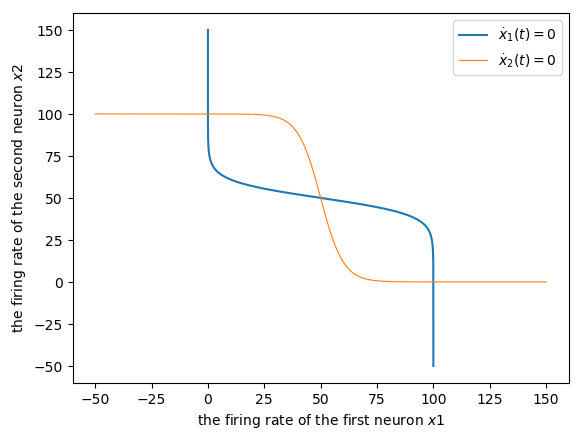
\includegraphics[width=0.7\linewidth]{mutual1}
  \caption
    {The nullclines of the system of two mutual inhibitory neurons}
\end{figure}

We observe three crossing points of the the two lines. From left to right,
we name them respectively $z_1$, $z_2$ and $z_3$ (so $z_2 = (50,50)$).
These are the points such that $\dot{x}_1 = \dot{x}_2 = 0$. In other words,
they're the fixed points of the dynamics. The plane is then divided into six
zones and in each zone the system evolves in a specific direction. To put it
simply, on the left of the blue line we have $\dot{x}_1 > 0$ while on the
right $\dot{x}_1 < 0$. Similarly, below the orange line we get
$\dot{x}_2 > 0$ whereas above it $\dot{x}_2 < 0$.

To better undestand what this implies, we simulate the system and plot the 
evolution of the firing rates for different initial conditions in the figure 
below.

\begin{figure}[H]
  \centering
  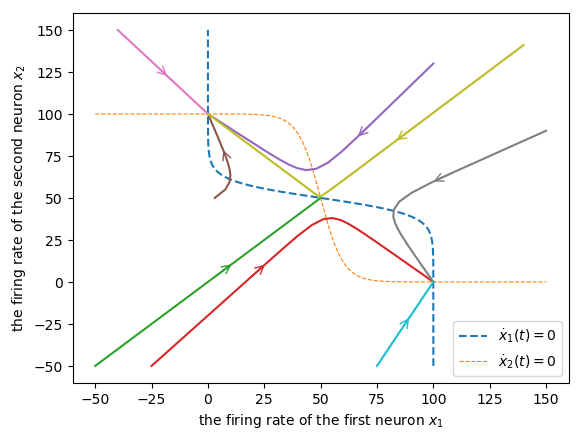
\includegraphics[width=0.7\linewidth]{mutual2}
  \caption
    {The evolution of the firing rates for different initial conditions}
\end{figure}

The initial conditions that are considered here are $(-50, -50)$, $(-40, 150)$,
$(-25, 50)$, $(3, 50)$, $(75, -50)$, $(100, 130)$, $(140, 141)$ and 
$(150, 90)$. First we notice that all of the simulations end up in some fixed
point and the directions of the evolutions follow roughly what is described
above. Further, it seems that (but without rigorous mathematical proof here)
given the initial condition $(x(0),y(0))$, if $x(0) < y(0)$ the system evolves
to $z_1$; if $x(0) = y(0)$ the system converges to $z_2$; finally if 
$x(0) > y(0)$ the system moves to $z_3$.

The yellow arrow serves as quite a good example: the initial condition is 
$(150, 151)$, and the system gets once very clear to $z_2$ but then it again
leaves away from this point and converges to $z_1$ at the end. As a result,
being fixed point, $z_1$ and $z_3$ are stable while $z_2$ is unstable. 
Finally, a plot of the vector field of derivatives can better 
explain all of this.

\begin{figure}[H]
  \centering
  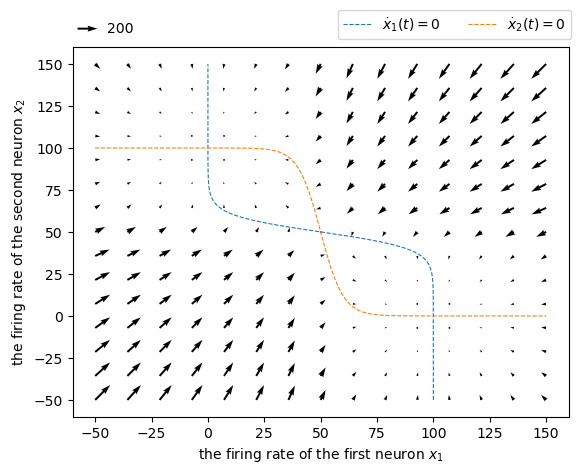
\includegraphics[width=0.7\linewidth]{mutual3}
  \caption{Derivatives at some points of the system}
\end{figure}

\subsection{Conclusion}

In this section, we have investigated two relatively simple networks and spent
time studying their dynamics. Several simulations have also been carried out.
We saw that there were diffrent kinds of fixed points of dynamics and if the
external currents were constant, the system would evolve towards some final 
state (which was often an attractor). Finally, the presence of noise may more
or less affect the evolution of the system.


\section{Hopfield Network}

\subsection{Description}

In the rest of the report we'll be interested in the continuous Hopfield 
model. The dynamics of the network is given the differential equation

\[\dot{\mathbf{x}} = -\mathbf{x}(t) + f(\mathbf{Wx}(t) + 
  \sigma\mathbf{\eta}(t)).\]

\noindent
The vector notation is adopted and a noise is also introduced.
Throughout the whole section, we set the dimension of $\mathbf{x}$ to be 
$N=64$ and thus $\mathbf{W}$ is a $64\times64$ matrix. For the sake of 
simplicity, we will take $f(x) = \mathrm{sgn}(x)$ for the moment being, and 
we use the convention that $\mathrm{sgn}(0) = 0$. As a result, $\mathbf{x}$
is typically a vector of reels between -1 and 1.

A such network can act as an associative memory system. For example, to store
one pattern $\mathbf{p}$ we set the weight matrix to 

\[\mathbf{W} = \frac{1}{N} \mathbf{p}\mathbf{p}^{\top}.\]

\noindent
Then it's quite easy to see that $\mathbf{p}$ is a fixed point of the
dynamics. For illustration purpose, we'll plot the activity of the neurons
as a figure containing $[8 \times 8]$ cases.

\subsection{Simulations}

To start we say that the network is meant to store just one pattern 
(\autoref{fig: Hopfield_one} - \textsf{A}) and the
noise level is $\sigma = 0.1$. As shown in \autoref{fig: Hopfield_one} -
\textsf{B}, the system may converge to $\mathbf{p}$. However, chances are 
that the it evolves towards $-\mathbf{p}$ 
(\autoref{fig: Hopfield_one} - \textsf{C}). We can easily show
that $-\mathbf{p}$ is indeed also a fixed point of the dynamics, but since
it's not a pattern that we aim to store, it's called a spurious state.
Looking at the differential equation, one may notice that there is still
another fixed point of the system: when $\mathbf{x} = \mathbf{0}$. 
Nonetheless, unlike the two previous fixed points, this one is not stable
and noise can bring the system away from it (\autoref{fig: Hopfield_one} -
\textsf{D}).

To store more patterns, say, $M$ patterns from $\mathbf{p}_1$ to 
$\mathbf{p}_M$, the general rule is to construct the weight matrix as

\[\mathbf{W} = \frac{1}{N} \sum_{i=1}^M \mathbf{p}_i\mathbf{p}_i^{\top}.\]

\noindent
For example in \autoref{fig: Hopfield_two} we store two patterns $\mathbf{p}$
and $\mathbf{q}$ in the network. We start from 
initial conditions that are respectively ``close'' to $\mathbf{p}$,
$-\mathbf{p}$, $\mathbf{q}$ and $-\mathbf{q}$. By close we mean that we change
the activity of a relative small number of neurons its opposite value 
(from 1 to -1 and from -1 to 1). We see that the network is always able
to evolve to the right fixed point.

However, surely we cannot store an unlimited number of patterns in the 
network. The network capcity depends on the explicit patterns that we want
to store. In \autoref{fig: Hopfield_six} we try to store six different 
patterns in the Hopfield network, but it doen't work perfectly.
In \autoref{fig: Hopfield_six} - \textsf{B} we start from a state that is
close to the first pattern we'd like to store and we manage to retrieve it
at the end. On the contrary, sometimes even though the initial condition 
is very similar to one of the stored patterns, we may fail to converge to 
this pattern and ends up in a state that is neither stored nor opposite of 
one that should be stored in our network (\autoref{fig: Hopfield_six} -
\textsf{C}, the initial condition is close to the fifth pattern we aim to
store).

If we start from a random initial state, the network may converge to
a stored pattern (\autoref{fig: Hopfield_six} - \textsf{D}), but as
described above, it can also evolve towards an arbitrary spurious state
that cannot be directly predicted from the stored patterns
(\autoref{fig: Hopfield_six} - \textsf{E, F}). Moreover, the convergence
might take a longer time and sometimes is not as direct as before 
(\autoref{fig: Hopfield_six} - \textsf{D}, the network finally converges
to the second stored pattern though showing only 50 simulation steps it may 
not yet be totally clear).

\newpage
\null
\vfill
\begin{figure}[H]
  \centering
  %
  \begin{subfigure}{0.28\textwidth}
    \centering
    
\includegraphics[width=\textwidth]{one_p0}
    \textsf{A}
  \end{subfigure}
  %
  \hspace{0.7em}
  %
  \begin{minipage}{0.62\textwidth}
    \begin{subfigure}{\textwidth}
      \textsf{B}
      \centering
      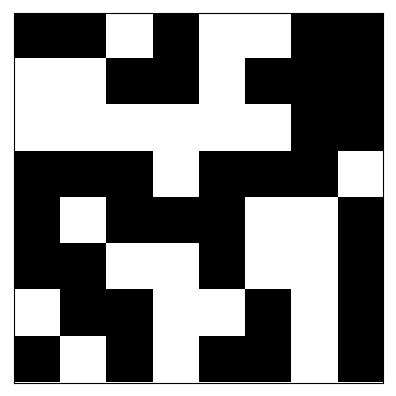
\includegraphics[width=0.18\textwidth]{one_4_0}
      
\includegraphics[width=0.18\textwidth]{one_4_1}
      
\includegraphics[width=0.18\textwidth]{one_4_2}
      
\includegraphics[width=0.18\textwidth]{one_4_3}
      
\includegraphics[width=0.18\textwidth]{one_4_4}
    \end{subfigure}\\[0.6em]
    %
    \begin{subfigure}{\textwidth}
      \textsf{C}
      \centering
      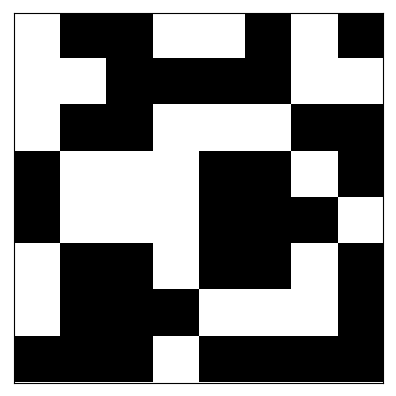
\includegraphics[width=0.18\textwidth]{one_3_0}
      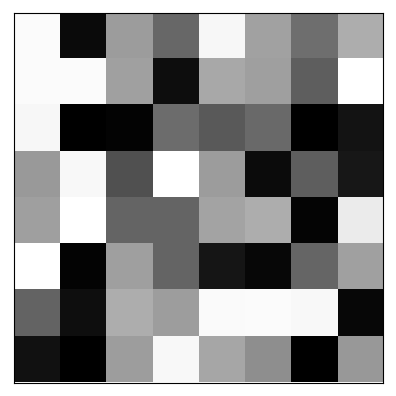
\includegraphics[width=0.18\textwidth]{one_3_1}
      
\includegraphics[width=0.18\textwidth]{one_3_2}
      
\includegraphics[width=0.18\textwidth]{one_3_3}
      
\includegraphics[width=0.18\textwidth]{one_3_4}
    \end{subfigure}\\[0.6em]
    %
    \begin{subfigure}{\textwidth}
      \textsf{D}
      \centering
      
\includegraphics[width=0.18\textwidth]{one_0_0}
      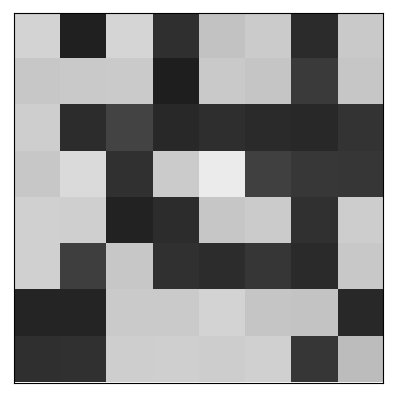
\includegraphics[width=0.18\textwidth]{one_0_1}
      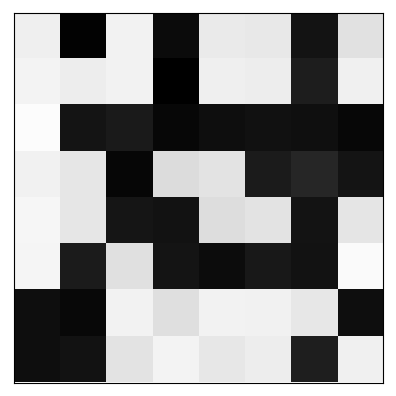
\includegraphics[width=0.18\textwidth]{one_0_2}
      
\includegraphics[width=0.18\textwidth]{one_0_3}
      
\includegraphics[width=0.18\textwidth]{one_0_4}
    \end{subfigure}
    %
  \end{minipage}
  \vspace{1.2em}
  \caption{Store one pattern in a Hopfield network.
           \textsf{A.} The stored pattern.
           \textsf{B.C.D.} Simulations with different initial conditions
           (between two successive picutres we carry out 10 steps of
           simulation).}
  \label{fig: Hopfield_one}
\end{figure}

\vfill

\begin{figure}[H]
  \centering
  %
  \begin{minipage}{0.275\textwidth}
    \begin{subfigure}{\textwidth}
      \centering
      
\includegraphics[width=\textwidth]{two_p0}
      \textsf{A}
    \end{subfigure}\\[0.3em]
    %
    \begin{subfigure}{\textwidth}
      \centering
      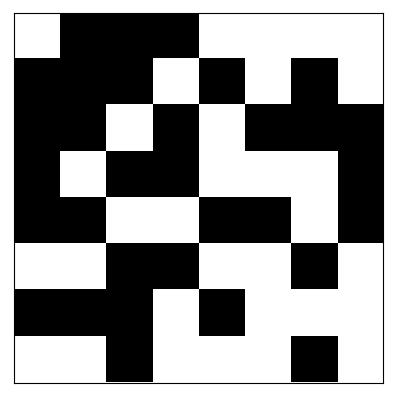
\includegraphics[width=\textwidth]{two_p1}
      \textsf{B}
    \end{subfigure}
  \end{minipage}
  %
  \hspace{0.7em}
  %
  \begin{minipage}{0.62\textwidth}
    \begin{subfigure}{\textwidth}
      \textsf{C}
      \centering
      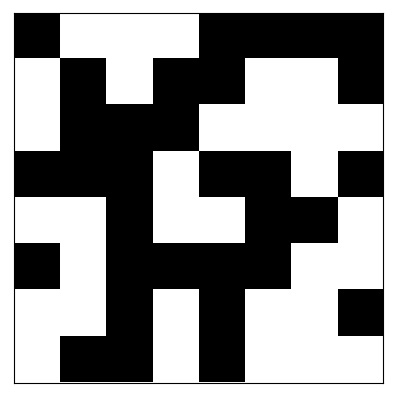
\includegraphics[width=0.22\textwidth]{two_1_0}
      
\includegraphics[width=0.22\textwidth]{two_1_1}
      
\includegraphics[width=0.22\textwidth]{two_1_2}
      
\includegraphics[width=0.22\textwidth]{two_1_3}
    \end{subfigure}\\[0.8em]
    %
    \begin{subfigure}{\textwidth}
      \textsf{D}
      \centering
      
\includegraphics[width=0.22\textwidth]{two_2_0}
      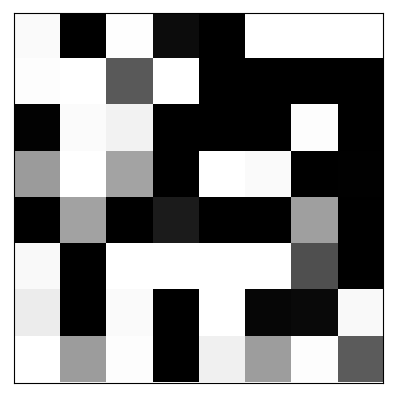
\includegraphics[width=0.22\textwidth]{two_2_1}
      
\includegraphics[width=0.22\textwidth]{two_2_2}
      
\includegraphics[width=0.22\textwidth]{two_2_3}
    \end{subfigure}\\[0.8em]
    %
    \begin{subfigure}{\textwidth}
      \textsf{E}
      \centering
      
\includegraphics[width=0.22\textwidth]{two_3_0}
      
\includegraphics[width=0.22\textwidth]{two_3_1}
      
\includegraphics[width=0.22\textwidth]{two_3_2}
      
\includegraphics[width=0.22\textwidth]{two_3_3}
    \end{subfigure}\\[0.8em]
    %
    \begin{subfigure}{\textwidth}
      \textsf{F}
      \centering
      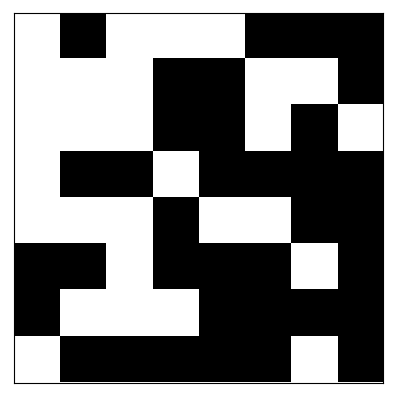
\includegraphics[width=0.22\textwidth]{two_4_0}
      
\includegraphics[width=0.22\textwidth]{two_4_1}
      
\includegraphics[width=0.22\textwidth]{two_4_2}
      
\includegraphics[width=0.22\textwidth]{two_4_3}
    \end{subfigure}
    %
  \end{minipage}
  \vspace{1.2em}
  \caption{Store two patterns in a Hopfield network.
           \textsf{A.B.} Stored patterns.
           \textsf{C.D.E.F.} Simulations with different initial conditions
           that are close to stored patterns or their opposites.}
  \label{fig: Hopfield_two}
\end{figure}
\vfill

\newpage

\null
\vfill

\begin{figure}[H]
  \centering
  \begin{subfigure}{\textwidth}
    \textsf{A}
    \centering
    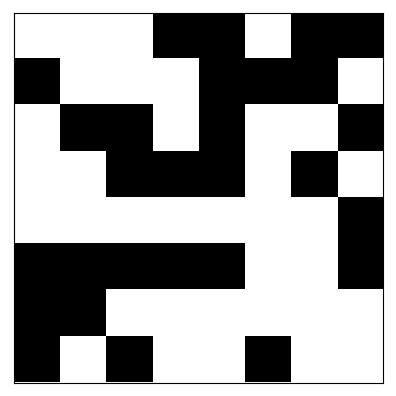
\includegraphics[width=0.15\textwidth]{six_p0}
    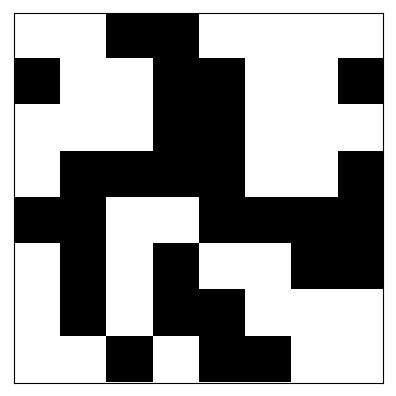
\includegraphics[width=0.15\textwidth]{six_p1}
    
\includegraphics[width=0.15\textwidth]{six_p2}
    
\includegraphics[width=0.15\textwidth]{six_p3}
    \includegraphics[width=0.15\textwidth]{six_p4}
    \includegraphics[width=0.15\textwidth]{six_p5}
  \end{subfigure}\\[1em]
  %
  \hspace{1em}\rule{0.95\textwidth}{1.8pt}\\
  \vspace{1em}
  %
  \begin{subfigure}{\textwidth}
    \textsf{B}
    \centering
    \includegraphics[width=0.15\textwidth]{six_1_0}
    \includegraphics[width=0.15\textwidth]{six_1_1}
    \includegraphics[width=0.15\textwidth]{six_1_2}
    \includegraphics[width=0.15\textwidth]{six_1_3}
    \includegraphics[width=0.15\textwidth]{six_1_4}
    \includegraphics[width=0.15\textwidth]{six_1_5}
  \end{subfigure}\\[0.8em]
  %
  \begin{subfigure}{\textwidth}
    \textsf{C}
    \centering
    \includegraphics[width=0.15\textwidth]{six_9_0}
    \includegraphics[width=0.15\textwidth]{six_9_1}
    \includegraphics[width=0.15\textwidth]{six_9_2}
    \includegraphics[width=0.15\textwidth]{six_9_3}
    \includegraphics[width=0.15\textwidth]{six_9_4}
    \includegraphics[width=0.15\textwidth]{six_9_5}
  \end{subfigure}\\[0.8em]
  %
  \begin{subfigure}{\textwidth}
    \textsf{D}
    \centering
    \includegraphics[width=0.15\textwidth]{six_13_0}
    \includegraphics[width=0.15\textwidth]{six_13_1}
    \includegraphics[width=0.15\textwidth]{six_13_2}
    \includegraphics[width=0.15\textwidth]{six_13_3}
    \includegraphics[width=0.15\textwidth]{six_13_4}
    \includegraphics[width=0.15\textwidth]{six_13_5}
  \end{subfigure}\\[0.8em]
  %
  \begin{subfigure}{\textwidth}
    \textsf{E}
    \centering
    \includegraphics[width=0.15\textwidth]{six_8_0}
    \includegraphics[width=0.15\textwidth]{six_8_1}
    \includegraphics[width=0.15\textwidth]{six_8_2}
    \includegraphics[width=0.15\textwidth]{six_8_3}
    \includegraphics[width=0.15\textwidth]{six_8_4}
    \includegraphics[width=0.15\textwidth]{six_8_5}
  \end{subfigure}\\[0.8em]
  %
  \begin{subfigure}{\textwidth}
    \textsf{F}
    \centering
    \includegraphics[width=0.15\textwidth]{six_16_0}
    \includegraphics[width=0.15\textwidth]{six_16_1}
    \includegraphics[width=0.15\textwidth]{six_16_2}
    \includegraphics[width=0.15\textwidth]{six_16_3}
    \includegraphics[width=0.15\textwidth]{six_16_4}
    \includegraphics[width=0.15\textwidth]{six_16_5}
  \end{subfigure}
  \vspace{1.2em}
  \caption{Try to store six patterns in a Hopfield network.
           \textsf{A.} Stored patterns.
           \textsf{B.C.D.E.} Simulations with different initial conditions.}
  \label{fig: Hopfield_six}
\end{figure}

\vfill

\newpage

Now how about replacing sgn by tanh for the activation function? To simplify
the task, we'll first remove noise from the network and we attempt to
store only one pattern in the network. As shown in 
\autoref{fig: Hopfield_tanh},
the values of final states are proportional to those of $\mathbf{p}$,
but neuron activities are in general of much smaller magnitude. The 
convergence is also much slower. 

It's easy to imagine that in this case, the presence of noise can degrade
severely the performance of the network. Indeed when we put again
$\sigma=0.1$, the result is shown in \autoref{fig: Hopfield_tanh_noise}. 
Neuron activities seem to be pure noise and we can hardly retrieve any
information from it (notice that until now for the same simulation in
one figure two successive images are separated by 10 simulation steps
while from now on they'll be separated by 50 simulation steps).

The problem becomes even more complex if we store several patterns in 
the network. Again we'll remove noise from the model and this time we want
to store two patterns in the network. Several scenarios can occur: the
network may just work as before except a final state with much lower 
activity level (\autoref{fig: Hopfield_tanh_two}); however, chances are
the two stored patterns are no longer fixed points of the dynamics and
even starting from the stored patterns we fall into another state that
doesnt't appear to be reltated to what we want to store 
(\autoref{fig: Hopfield_tanh_two2}). We notice also that the convergence
of the system takes much more long time.

\subsection{Conclusion}
With the differential equation that is given at the beginning of the
section and the general rule used to generate the weight matrix, 
we have simulated the dynamics of the network under various situations. 
We saw that when $f = \mathrm{sgn}$ and if we stored just a small number
of patterns the Hopfield network could act correctly as an associative 
memory despite the presence of noise.
However the network capacity is without doubt limited and many spurious
states could appear if we tried to store too many patterns in a network.

When $f = \tanh$, the dynamics of the system seems to be more complicated.
The values of the final states are much closer to 0, noise can be fatal to
the system, the convergence is much slower and unexpected attractors
may appear when we want to store more than one patterns.

We didn't do any mathematical proofs in this section, but to study more
in details the Hopfield network, new notions must be introduced (e.g.
energy of the network) and this will be a topic much more complex and
beyond the scope of this report.

\begin{figure}[H]
  \centering
  %
  \begin{subfigure}{0.26\textwidth}
    \centering
    \includegraphics[width=\textwidth]{tanh_p0}
    \textsf{A}
  \end{subfigure}
  %
  \hspace{0.7em}
  %
  \begin{minipage}{0.64\textwidth}
    \begin{subfigure}{\textwidth}
      \textsf{B}
      \centering
      \includegraphics[width=0.15\textwidth]{tanh_1_0}
      \includegraphics[width=0.15\textwidth]{tanh_1_1}
      \includegraphics[width=0.15\textwidth]{tanh_1_2}
      \includegraphics[width=0.15\textwidth]{tanh_1_3}
      \includegraphics[width=0.15\textwidth]{tanh_1_4}
      \includegraphics[width=0.15\textwidth]{tanh_1_5}
    \end{subfigure}\\[0.6em]
    %
    \begin{subfigure}{\textwidth}
      \textsf{C}
      \centering
      \includegraphics[width=0.15\textwidth]{tanh_3_0}
      \includegraphics[width=0.15\textwidth]{tanh_3_1}
      \includegraphics[width=0.15\textwidth]{tanh_3_2}
      \includegraphics[width=0.15\textwidth]{tanh_3_3}
      \includegraphics[width=0.15\textwidth]{tanh_3_4}
      \includegraphics[width=0.15\textwidth]{tanh_3_5}
    \end{subfigure}\\[0.6em]
    %
    \begin{subfigure}{\textwidth}
      \textsf{D}
      \centering
      \includegraphics[width=0.15\textwidth]{tanh_5_0}
      \includegraphics[width=0.15\textwidth]{tanh_5_1}
      \includegraphics[width=0.15\textwidth]{tanh_5_2}
      \includegraphics[width=0.15\textwidth]{tanh_5_3}
      \includegraphics[width=0.15\textwidth]{tanh_5_4}
      \includegraphics[width=0.15\textwidth]{tanh_5_5}
    \end{subfigure}
    %
  \end{minipage}
  \vspace{1.2em}
  \caption{Store one pattern in a Hopfield network with $f = \tanh$ 
           without noise.
           \textsf{A.} The stored pattern.
           \textsf{B.C.D.} Simulations with random initial conditions.}
  \label{fig: Hopfield_tanh}

\end{figure}

\newpage
\null
\vfill

\begin{figure}[H]
  \centering
  %
  \begin{subfigure}{\textwidth}
    \hspace{0.6em}
    \textsf{A}
    \includegraphics[width=0.11\textwidth]{tanh_p0}
  \end{subfigure}\\[1em]
  %
  \hspace*{1.2em}\rule{0.95\textwidth}{1.8pt}\\[1em]
  %
  \begin{subfigure}{\textwidth}
    \hspace{0.6em}
    \textsf{B}
    \includegraphics[width=0.11\textwidth]{tanh_noise_1_0}
    \includegraphics[width=0.11\textwidth]{tanh_noise_1_1}
    \includegraphics[width=0.11\textwidth]{tanh_noise_1_2}
    \includegraphics[width=0.11\textwidth]{tanh_noise_1_3}
    \includegraphics[width=0.11\textwidth]{tanh_noise_1_4}
    \includegraphics[width=0.11\textwidth]{tanh_noise_1_5}
    \includegraphics[width=0.11\textwidth]{tanh_noise_1_6}
    \includegraphics[width=0.11\textwidth]{tanh_noise_1_7}
  \end{subfigure}\\[0.6em]
  %
  \begin{subfigure}{\textwidth}
    \hspace{0.6em}
    \textsf{C}
    \includegraphics[width=0.11\textwidth]{tanh_noise_2_0}
    \includegraphics[width=0.11\textwidth]{tanh_noise_2_1}
    \includegraphics[width=0.11\textwidth]{tanh_noise_2_2}
    \includegraphics[width=0.11\textwidth]{tanh_noise_2_3}
    \includegraphics[width=0.11\textwidth]{tanh_noise_2_4}
    \includegraphics[width=0.11\textwidth]{tanh_noise_2_5}
    \includegraphics[width=0.11\textwidth]{tanh_noise_2_6}
    \includegraphics[width=0.11\textwidth]{tanh_noise_2_7}
  \end{subfigure}
  %
  \vspace{1.2em}
  \caption{Store one pattern in a Hopfield network with $f = \tanh$ 
           with noise.
           \textsf{A.} The stored pattern.
           \textsf{B.C.} Simulations with random initial conditions
           (between two successive picutres we carry out 50 steps of
           simulation).}
  \label{fig: Hopfield_tanh_noise}

\end{figure}

\vfill

\begin{figure}[H]
  %
    \begin{subfigure}{\textwidth}
      \hspace{1em}
      \textsf{A}
      \includegraphics[width=0.15\textwidth]{tanh_two_p0}
      \includegraphics[width=0.15\textwidth]{tanh_two_p1}
    \end{subfigure}\\[1em]
  %
  \hspace*{2.2em}\rule{0.95\textwidth}{1.8pt}\\[1em]
  %
    \begin{subfigure}{\textwidth}
      \hspace{1em}
      \textsf{B}
      \includegraphics[width=0.15\textwidth]{tanh_two_6_0}
      \includegraphics[width=0.15\textwidth]{tanh_two_6_1}
      \includegraphics[width=0.15\textwidth]{tanh_two_6_2}
      \includegraphics[width=0.15\textwidth]{tanh_two_6_3}
      \includegraphics[width=0.15\textwidth]{tanh_two_6_4}
      \includegraphics[width=0.15\textwidth]{tanh_two_6_5}
    \end{subfigure}\\[0.6em]
    %
    \begin{subfigure}{\textwidth}
      \hspace{1em}
      \textsf{C}
      \includegraphics[width=0.15\textwidth]{tanh_two_7_0}
      \includegraphics[width=0.15\textwidth]{tanh_two_7_1}
      \includegraphics[width=0.15\textwidth]{tanh_two_7_2}
      \includegraphics[width=0.15\textwidth]{tanh_two_7_3}
      \includegraphics[width=0.15\textwidth]{tanh_two_7_4}
      \includegraphics[width=0.15\textwidth]{tanh_two_7_5}
    \end{subfigure}\\[0.6em]
    %
    \begin{subfigure}{\textwidth}
      \hspace{1em}
      \textsf{D}
      \includegraphics[width=0.15\textwidth]{tanh_two_9_0}
      \includegraphics[width=0.15\textwidth]{tanh_two_9_1}
      \includegraphics[width=0.15\textwidth]{tanh_two_9_2}
      \includegraphics[width=0.15\textwidth]{tanh_two_9_3}
      \includegraphics[width=0.15\textwidth]{tanh_two_9_4}
      \includegraphics[width=0.15\textwidth]{tanh_two_9_5}
    \end{subfigure}
    %
  \vspace{1.2em}
  \caption{Store two patterns in a Hopfield network with $f = \tanh$ 
           without noise, with success.
           \textsf{A.} Stored patterns.
           \textsf{B.C.D.} Simulations with random initial conditions.}
  \label{fig: Hopfield_tanh_two}

\end{figure}

\vfill

\newpage
\null
\vfill

\begin{figure}[H]
  %
    \begin{subfigure}{\textwidth}
      \hspace{1em}
      \textsf{A}
      \includegraphics[width=0.15\textwidth]{tanh_two2_p0}
      \includegraphics[width=0.15\textwidth]{tanh_two2_p1}
    \end{subfigure}\\[1em]
  %
  \hspace*{2.2em}\rule{0.95\textwidth}{1.8pt}\\[1em]
  %
    \begin{subfigure}{\textwidth}
      \hspace{2em}
      \includegraphics[width=0.15\textwidth]{tanh_two2_1_0}
      \includegraphics[width=0.15\textwidth]{tanh_two2_1_1}
      \includegraphics[width=0.15\textwidth]{tanh_two2_1_2}
      \includegraphics[width=0.15\textwidth]{tanh_two2_1_3}
      \includegraphics[width=0.15\textwidth]{tanh_two2_1_4}
      \includegraphics[width=0.15\textwidth]{tanh_two2_1_5}\\
      \hspace*{1em}
      \textsf{B}
      \includegraphics[width=0.15\textwidth]{tanh_two2_1_6}
      \includegraphics[width=0.15\textwidth]{tanh_two2_1_7}
      \includegraphics[width=0.15\textwidth]{tanh_two2_1_8}
      \includegraphics[width=0.15\textwidth]{tanh_two2_1_9}
      \includegraphics[width=0.15\textwidth]{tanh_two2_1_10}
      \includegraphics[width=0.15\textwidth]{tanh_two2_1_11}
    \end{subfigure}\\[0.6em]
    %
    \begin{subfigure}{\textwidth}
      \hspace{2em}
      \includegraphics[width=0.15\textwidth]{tanh_two2_3_0}
      \includegraphics[width=0.15\textwidth]{tanh_two2_3_1}
      \includegraphics[width=0.15\textwidth]{tanh_two2_3_2}
      \includegraphics[width=0.15\textwidth]{tanh_two2_3_3}
      \includegraphics[width=0.15\textwidth]{tanh_two2_3_4}
      \includegraphics[width=0.15\textwidth]{tanh_two2_3_5}\\
      \hspace*{1em}
      \textsf{C}
      \includegraphics[width=0.15\textwidth]{tanh_two2_3_6}
      \includegraphics[width=0.15\textwidth]{tanh_two2_3_7}
      \includegraphics[width=0.15\textwidth]{tanh_two2_3_8}
      \includegraphics[width=0.15\textwidth]{tanh_two2_3_9}
      \includegraphics[width=0.15\textwidth]{tanh_two2_3_10}
      \includegraphics[width=0.15\textwidth]{tanh_two2_3_11}
    \end{subfigure}\\[0.6em]
    %
    \begin{subfigure}{\textwidth}
      \hspace{2em}
      \includegraphics[width=0.15\textwidth]{tanh_two2_8_0}
      \includegraphics[width=0.15\textwidth]{tanh_two2_8_1}
      \includegraphics[width=0.15\textwidth]{tanh_two2_8_2}
      \includegraphics[width=0.15\textwidth]{tanh_two2_8_3}
      \includegraphics[width=0.15\textwidth]{tanh_two2_8_4}
      \includegraphics[width=0.15\textwidth]{tanh_two2_8_5}\\
      \hspace*{1em}
      \textsf{D}
      \includegraphics[width=0.15\textwidth]{tanh_two2_8_6}
      \includegraphics[width=0.15\textwidth]{tanh_two2_8_7}
      \includegraphics[width=0.15\textwidth]{tanh_two2_8_8}
      \includegraphics[width=0.15\textwidth]{tanh_two2_8_9}
      \includegraphics[width=0.15\textwidth]{tanh_two2_8_10}
      \includegraphics[width=0.15\textwidth]{tanh_two2_8_11}
    \end{subfigure}\\[0.6em]
    %
  \vspace{1.2em}
  \caption{Store two patterns in a Hopfield network with $f = \tanh$ 
           without noise, new fixed points appear instead of the stored ones.
           \textsf{A.} Stored patterns.
           \textsf{B.C.} Simulations starting from stored patterns.
           \textsf{D.} Simulations with random initial condition.}
  \label{fig: Hopfield_tanh_two2}

\end{figure}

\vfill

\end{document}
